\documentclass[]{standalone}
\usepackage{tikz}
\begin{document}
  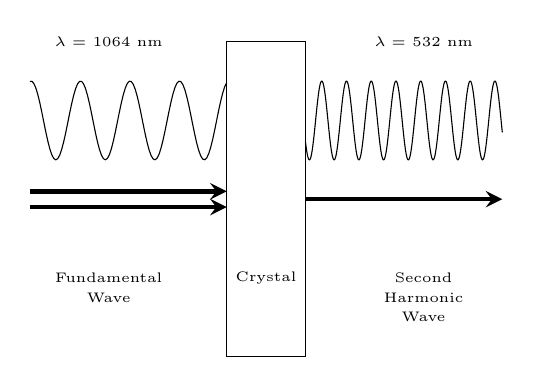
\begin{tikzpicture}
	  \draw[] (-.5,-2) rectangle (.5,2);
	  \draw[samples = 100, domain = -3:-.5]   plot (\x,{.5*sin(10 * \x r)+1}) ;
	  \draw[samples = 1000, domain = .5:3]   plot (\x,{.5*sin(20 * \x r)+1}) ;
	  \draw[->,>=stealth, line width = 1.6pt] (-3,.1) -- (-.5,.1);
	  \draw[->,>=stealth, line width = 1.6pt] (-3,-.1) -- (-.5,-.1);
	  \draw[->,>=stealth, line width = 1.6pt] (.5,0) -- (3,0);
	  \node at (-2,2) {\tiny $\lambda = $ 1064 nm};
	  \node at (2,2) {\tiny $\lambda = $ 532 nm};
	  \node at (-2,-1) {\tiny Fundamental};
	  \node at (-2,-1.25) {\tiny Wave};
	  \node at (2,-1) {\tiny Second};
	  \node at (2,-1.25) {\tiny Harmonic};
	  \node at (2,-1.5) {\tiny Wave};
	  \node at (0,-1) {\tiny Crystal};
  \end{tikzpicture}
\end{document}
